\input{presentacion.tex}

\begin{document}

{\setbeamercolor{background canvas}{bg=}
	
	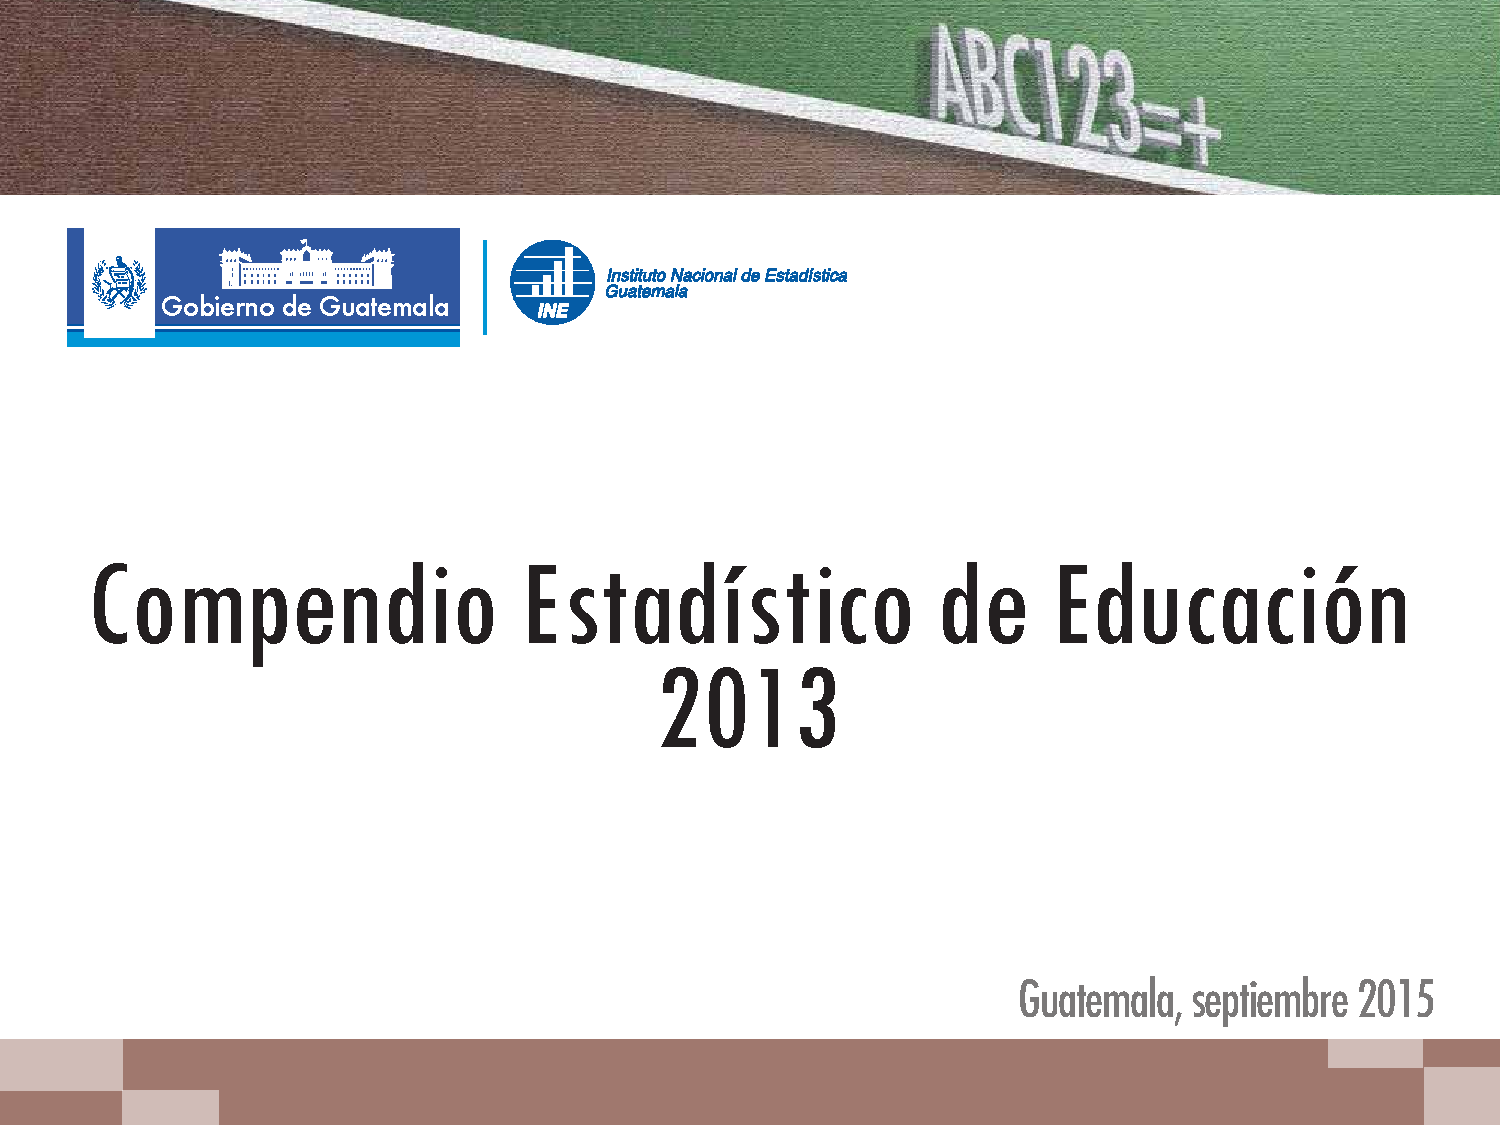
\includepdf{diapositiva_educativa.pdf}}

\INEchaptercarta{Alumnos en preprimaria}{}



\cajita{Inscritos }{El número de  inscritos en preprimaria, se obtiene a partir del total de los alumnos que tienen hasta seis años, registrados al treinta de marzo de cada ciclo escolar\llamada. \textollamada{También se le llama estadística inicial} 
	
	En el 2009 se inscribieron 584,833 alumnos y en el 2014 se inscribieron 543,226 alumnos, lo cual representa un crecimiento de 13.7\%.}{Número de inscritos en el ciclo de educación preprimaria}{República de Guatemala, serie histórica, en datos absolutos}{\ \\[0mm]\begin{tikzpicture}[x=1pt,y=1pt, scale=.8]  \input{C:/Users/INE/Desktop/compendio_educacion/graficas/preprimaria/}  \end{tikzpicture}}{Instituto Nacional de Estadística, con datos del Ministerio de Educación}

\cajita{Inscritos por etnia}{La distribución de alumnos inscritos en educación preprimaria según su etnicidad, muestra que el 72.9\% fueron no indígenas.}{Distribución de inscritos en el ciclo de\\ educación preprimaria, por grupo étnico}{República de Guatemala, año 2014, en porcentaje}{\ \\[0mm]\begin{tikzpicture}[x=1pt,y=1pt, scale=.8]  \input{C:/Users/INE/Desktop/compendio_educacion/graficas/preprimaria/}  \end{tikzpicture}}{Instituto Nacional de Estadística, con datos del Ministerio de Educación}


\cajita{Inscritos por sector educativo}{La distribución de alumnos inscritos en educación preprimaria muestra que el 83\%  el porcentaje alumnos inscritos en preprimaria  en el en el sector privado es de 83.5\%.}{Distribución de inscritos en el ciclo de educación preprimaria,\\ por sector educativo}{República de Guatemala, año 2014, en porcentaje}{\ \\[0mm]\begin{tikzpicture}[x=1pt,y=1pt, scale=.8]  \input{C:/Users/INE/Desktop/compendio_educacion/graficas/preprimaria/}  \end{tikzpicture}}{Instituto Nacional de Estadística, con datos del Ministerio de Educación}

\cajita{Inscritos e idioma}{Del total de alumnos inscritos en preprimaria, el 85.2\% reciben clases en idioma español.}{Distribución de inscritos en el ciclo de educación preprimaria, según el idioma en el que reciben clases}{República de Guatemala, año 2014, en porcentaje}{\ \\[0mm]\begin{tikzpicture}[x=1pt,y=1pt, scale=.8]  \input{C:/Users/INE/Desktop/compendio_educacion/graficas/preprimaria/}  \end{tikzpicture}}{Instituto Nacional de Estadística, con datos del Ministerio de Educación}



\INEchaptercarta{Indicadores de preprimaria}{}



\cajita{Cobertura neta}{ La tasa neta, es la relación que existe entre la parte de la inscripción inicial que se encuentra en la edad escolar hasta de 6 años y la población en edad escolar hasta 6 años.
	
	La tasa neta de cobertura en preprimaria, presentó el año 2009 el 57.1\% en el año 2014 fue de 46.2\%, que representó un decrecimiento del 19\% respecto del 2009.}{Tasa neta de cobertura del ciclo de educación preprimaria}{República de Guatemala, serie histórica, en porcentaje}{\ \\[0mm]\begin{tikzpicture}[x=1pt,y=1pt, scale=.8]  \input{C:/Users/INE/Desktop/compendio_educacion/graficas/preprimaria/}  \end{tikzpicture}}{Instituto Nacional de Estadística, con datos del Ministerio de Educación}

\cajota{Cobertura neta en los departamentos}{Los departamentos con la menor tasa neta de cobertura en preprimaria fueron: Quiché 29.4\%, Totonicapán 32.6\% y Alta Verapaz con 34.8\%. 	Los departamentos donde hubo alta tasa neta de cobertura en preprimaria fueron: Zacapa 59.5\%, El Progreso 59.7\% y Guatemala 66.4\%.}{Tasa neta de cobertura del ciclo de educación preprimaria}{Por departamento, año 2014, en porcentaje}{\includegraphics[height=2.6in]{C:/Users/INE/Desktop/compendio_educacion/graficas/preprimaria/}}{Instituto Nacional de Estadística, con datos del Ministerio de Educación}

 % % % % % % % % % %

\INEchaptercarta{Alumnos en primaria}{}



\cajita{Inscritos en primaria }{El número de  inscritos en primaria, se obtiene a partir del total de los alumnos que tienen hasta doce años, registrados al treinta de marzo de cada año escolar.  
	
	En la presente gráfica en serie de años, se observa que en el año 2009 se inscribieron 2,659,776 alumnos y en el año 2014 se inscribieron 2,476,379 alumnos, lo cual muestra un decrecimiento de 6.9\%.}{Número de inscritos en el ciclo de educación primaria}{República de Guatemala, serie histórica, en datos absolutos}{\ \\[0mm]\begin{tikzpicture}[x=1pt,y=1pt, scale=.8]  \input{C:/Users/INE/Desktop/compendio_educacion/graficas/primaria/}  \end{tikzpicture}}{Instituto Nacional de Estadística, con datos del Ministerio de Educación}

\cajita{Inscritos en primaria por sexo}{En la presente gráfica, se observa que el porcentaje de hombres inscritos en primaria es 51.7\% y de mujeres  48.3\% siendo la diferencia de 3.4 puntos porcentuales.}{Distribución de inscritos en el ciclo de educación primaria, por sexo}{República de Guatemala, año 2014, en porcentaje}{\ \\[0mm]\begin{tikzpicture}[x=1pt,y=1pt, scale=.8]  \input{C:/Users/INE/Desktop/compendio_educacion/graficas/primaria/}  \end{tikzpicture}}{Instituto Nacional de Estadística, con datos del Ministerio de Educación}

\cajita{Inscritos en primaria por grado}{En la presente gráfica, se observa el número de inscritos por grado en primaria y se observa que donde se concentra la mayor cantidad de alumnos es en primer grado, con el 20.3\% y donde menos inscritos hay, es en sexto grado con 13.4\%.}{Número de inscritos en el ciclo de educación primaria, \\ según el grado escolar}{República de Guatemala, año 2014, en porcentaje}{\ \\[0mm]\begin{tikzpicture}[x=1pt,y=1pt, scale=.8]  \input{C:/Users/INE/Desktop/compendio_educacion/graficas/primaria/}  \end{tikzpicture}}{Instituto Nacional de Estadística, con datos del Ministerio de Educación}



\cajita{Inscritos en primaria por sector educativo}{En la presente gráfica, se observa que del total de inscritos en primaria, el 89.2\% están inscritos en el sector público.}{Distribución de inscritos en el ciclo de educación primaria,\\ por sector educativo}{República de Guatemala, año 2014, en porcentaje}{\ \\[0mm]\begin{tikzpicture}[x=1pt,y=1pt, scale=.8]  \input{C:/Users/INE/Desktop/compendio_educacion/graficas/primaria/}  \end{tikzpicture}}{Instituto Nacional de Estadística, con datos del Ministerio de Educación}




\INEchaptercarta{Indicadores de educación primaria}{}


\cajita{Cobertura neta}{La tasa neta de cobertura en primaria, presentó el año 2009 el 98.7\% y en el año 2014 fue de 85.4\%, presentando un decrecimiento del 13.5\%.}{Tasa neta de cobertura del ciclo de educación primaria}{República de Guatemala, serie histórica, en porcentaje}{\ \\[0mm]\begin{tikzpicture}[x=1pt,y=1pt, scale=.8]  \input{C:/Users/INE/Desktop/compendio_educacion/graficas/primaria/}  \end{tikzpicture}}{Instituto Nacional de Estadística, con datos del Ministerio de Educación}


\cajota{Cobertura neta en los departamentos}{En el siguiente mapa se observan los departamentos donde hubo menor tasa neta de cobertura en primaria, siendo los siguientes: Petén 68\%, Totonicapán 74.2\% y Sololá 75.9.  Los departamentos donde hubo alta tasa neta de cobertura en primaria fueron: Zacapa 93.2\%, Retalhuleu 93.6 y San Marcos 93.8\% .El departamento de Guatemala presentó una tasa de  91.3\%. }{Tasa neta de cobertura del ciclo de educación primaria}{Por departamento, año 2014, en porcentaje}{\includegraphics[height=2.6in]{C:/Users/INE/Desktop/compendio_educacion/graficas/primaria/}}{Instituto Nacional de Estadística, con datos del Ministerio de Educación}




\cajita{Repitencia}{La tasa de repitencia en primaria, presentó el año 2009 el 11.5\% y en el año 2014 fue de 10.2\%, presentando un decrecimiento del 11.3\%.}{Tasa de repitencia del ciclo de educación primaria}{República de Guatemala, serie histórica, en porcentaje}{\ \\[0mm]\begin{tikzpicture}[x=1pt,y=1pt, scale=.8]  \input{C:/Users/INE/Desktop/compendio_educacion/graficas/primaria/}  \end{tikzpicture}}{Instituto Nacional de Estadística, con datos del Ministerio de Educación}

\cajita{Repitencia por sexo}{La tasa de repitencia en primaria por sexo, representa el 11.2\% para hombres y 9.2\% para las mujeres.}{Tasa de repitencia del ciclo de educación primaria, por sexo}{República de Guatemala, año 2014, en porcentaje}{\ \\[0mm]\begin{tikzpicture}[x=1pt,y=1pt, scale=.8]  \input{C:/Users/INE/Desktop/compendio_educacion/graficas/primaria/}  \end{tikzpicture}}{Instituto Nacional de Estadística, con datos del Ministerio de Educación}



\cajita{Sobre-edad}{La tasa de sobre-edad en primaria, presentó el año 2009 el 51.7\% y en el año 2014 fue de 20.8\%, presentando un decrecimiento del 59.8\%.}{Tasa de sobre-edad del ciclo de educación primaria}{República de Guatemala, serie histórica, en porcentaje}{\ \\[0mm]\begin{tikzpicture}[x=1pt,y=1pt, scale=.8]  \input{C:/Users/INE/Desktop/compendio_educacion/graficas/primaria/}  \end{tikzpicture}}{Instituto Nacional de Estadística, con datos del Ministerio de Educación}

\cajita{Sobre-edad por sexo}{La tasa de sobre-edad en primaria por sexo, representa el 22.7\% para hombres y 18.7\% para las mujeres.}{Tasa de sobre-edad del ciclo de educación primaria, por sexo}{República de Guatemala, año 2014, en porcentaje}{\ \\[0mm]\begin{tikzpicture}[x=1pt,y=1pt, scale=.8]  \input{C:/Users/INE/Desktop/compendio_educacion/graficas/primaria/}  \end{tikzpicture}}{Instituto Nacional de Estadística, con datos del Ministerio de Educación}




\cajita{Deserción}{La tasa de deserción en primaria, presentó el año 2009 5.5\% y en el año 2014 fue de 3.5\%, presentando un decrecimiento de 3.5\%.}{Tasa de deserción del ciclo de educación primaria}{República de Guatemala, serie histórica, en porcentaje}{\ \\[0mm]\begin{tikzpicture}[x=1pt,y=1pt, scale=.8]  \input{C:/Users/INE/Desktop/compendio_educacion/graficas/primaria/}  \end{tikzpicture}}{Instituto Nacional de Estadística, con datos del Ministerio de Educación}

\cajita{Deserción por sexo}{La tasa de deserción en primaria por sexo, representa el 3.8\% para hombres y 3.1\% para las mujeres.}{Tasa de deserción del ciclo de educación primaria, por sexo}{República de Guatemala, año 2014, en porcentaje}{\ \\[0mm]\begin{tikzpicture}[x=1pt,y=1pt, scale=.8]  \input{C:/Users/INE/Desktop/compendio_educacion/graficas/primaria/}  \end{tikzpicture}}{Instituto Nacional de Estadística, con datos del Ministerio de Educación}


\cajita{Aprobación}{La tasa de aprobación en primaria, presentó el año 2009 el 86.4\% y en el año 2014 fue de 86.6\%, presentando un crecimiento de 0.2\%.}{Tasa de aprobación del ciclo de educación primaria}{República de Guatemala, serie histórica, en porcentaje}{\ \\[0mm]\begin{tikzpicture}[x=1pt,y=1pt, scale=.8]  \input{C:/Users/INE/Desktop/compendio_educacion/graficas/primaria/}  \end{tikzpicture}}{Instituto Nacional de Estadística, con datos del Ministerio de Educación}










 % % % % % % % %



\INEchaptercarta{Alumnos en básico}{}



\cajita{Inscritos en básico }{El número de  inscritos en básico, se obtiene a partir del total de los alumnos registrados al treinta de marzo de cada año escolar y que comprenden de trece a quince años.
	
	En la presente gráfica en serie de años, se observa que en el año 2009 se inscribieron 671,872 alumnos y en el año 2014 se inscribieron 764,415 alumnos, lo cual muestra un crecimiento de 13.8\%.}{Número de inscritos en el ciclo de educación básica}{República de Guatemala, serie histórica, en datos absolutos}{\ \\[0mm]\begin{tikzpicture}[x=1pt,y=1pt, scale=.8]  \input{C:/Users/INE/Desktop/compendio_educacion/graficas/basicos/}  \end{tikzpicture}}{Instituto Nacional de Estadística, con datos del Ministerio de Educación}

\cajita{Inscritos en básico por sexo}{En la presente gráfica, se observa que el porcentaje de hombres inscritos en básico es 53.7\% y de mujeres  46.3\% siendo la diferencia de 7.4 puntos porcentuales.}{Distribución de inscritos en el ciclo de educación básica, por sexo}{República de Guatemala, año 2014, en porcentaje}{\ \\[0mm]\begin{tikzpicture}[x=1pt,y=1pt, scale=.8]  \input{C:/Users/INE/Desktop/compendio_educacion/graficas/basicos/}  \end{tikzpicture}}{Instituto Nacional de Estadística, con datos del Ministerio de Educación}

\cajita{Inscritos en básico por grado}{En la presente gráfica, se observa el número de inscritos por grado en básico y se observa que donde se concentra la mayor cantidad de alumnos es en primer grado, con el 41.7\% y donde menos inscritos hay, es en tercer grado con 27.9\%.}{Distribución de inscritos en el ciclo de educación básica, según el grado escolar}{República de Guatemala, año 2014, en porcentaje}{\ \\[0mm]\begin{tikzpicture}[x=1pt,y=1pt, scale=.8]  \input{C:/Users/INE/Desktop/compendio_educacion/graficas/basicos/}  \end{tikzpicture}}{Instituto Nacional de Estadística, con datos del Ministerio de Educación}

\cajita{Inscritos en básico por etnia}{En la presente gráfica, se observa que del total de inscritos en básico, los no indígenas representan el 75.2\%.}{Distribución de inscritos en el ciclo de educación básica, por grupo étnico}{República de Guatemala, año 2014, en porcentaje}{\ \\[0mm]\begin{tikzpicture}[x=1pt,y=1pt, scale=.8]  \input{C:/Users/INE/Desktop/compendio_educacion/graficas/basicos/}  \end{tikzpicture}}{Instituto Nacional de Estadística, con datos del Ministerio de Educación}


\cajita{Inscritos en básico por sector educativo}{En la presente gráfica, se observa que del total de inscritos en básico, el 44.3\% están inscritos en el sector público y también figura el sector Cooperativa con 20.5\% de los estudiantes inscritos.}{Distribución de inscritos en el ciclo de educación básica, por sector educativo}{República de Guatemala, año 2014, en porcentaje}{\ \\[0mm]\begin{tikzpicture}[x=1pt,y=1pt, scale=.8]  \input{C:/Users/INE/Desktop/compendio_educacion/graficas/basicos/}  \end{tikzpicture}}{Instituto Nacional de Estadística, con datos del Ministerio de Educación}

\cajita{Inscritos en básico e idioma}{En la presente gráfica, se observa que del total de inscritos en básico, el 97.5\% reciben clases en idioma español.}{Distribución de inscritos en el ciclo de educación básica, según el idioma en el que reciben clases}{República de Guatemala, año 2014, en porcentaje}{\ \\[0mm]\begin{tikzpicture}[x=1pt,y=1pt, scale=.8]  \input{C:/Users/INE/Desktop/compendio_educacion/graficas/basicos/}  \end{tikzpicture}}{Instituto Nacional de Estadística, con datos del Ministerio de Educación}





\INEchaptercarta{Indicadores de educación básica}{}



\cajita{Cobertura neta}{La tasa neta de cobertura en básico, presentó en el año 2009 el 40.3\% y en el año 2014 fue de 44\%, presentando un crecimiento de 9.4\%.}{Tasa neta de cobertura del ciclo de educación básica}{República de Guatemala, serie histórica, en porcentaje}{\ \\[0mm]\begin{tikzpicture}[x=1pt,y=1pt, scale=.8]  \input{C:/Users/INE/Desktop/compendio_educacion/graficas/basicos/}  \end{tikzpicture}}{Instituto Nacional de Estadística, con datos del Ministerio de Educación}

\cajita{Cobertura neta por sexo}{La tasa neta de cobertura en básico por sexo, representa el 45.6\% para hombres y 42.5\% para las mujeres.}{Tasa neta de cobertura del ciclo de educación básica, por sexo}{República de Guatemala, año 2014, en porcentaje}{\ \\[0mm]\begin{tikzpicture}[x=1pt,y=1pt, scale=.8]  \input{C:/Users/INE/Desktop/compendio_educacion/graficas/basicos/}  \end{tikzpicture}}{Instituto Nacional de Estadística, con datos del Ministerio de Educación}

\cajita{Cobertura neta en los departamentos}{En el siguiente mapa se observan los departamentos donde hubo menor tasa neta de cobertura en básico, fueron los siguientes: Alta Verapaz 22.6\%,  Quiché 24.7\% y Huehuetenango 25.7\%.\\
	
	Los departamentos donde hubo alta tasa neta de cobertura en básico fueron: Sacatepéquez 57.7\%, El Progreso 58\% y Guatemala 69.4\%. }{Tasa neta de cobertura del ciclo de educación básica}{Por departamento, año 2014, en porcentaje}{\includegraphics[height=2.6in]{C:/Users/INE/Desktop/compendio_educacion/graficas/basicos/}}{Instituto Nacional de Estadística, con datos del Ministerio de Educación}




 % % % % % % % % % % %



\INEchaptercarta{Alumnos en diversificado}{}



\cajita{Inscritos en diversificado }{El número de  inscritos en diversificado, se obtiene a partir del total de los alumnos registrados al treinta de marzo de cada año escolar, que comprenden las edades de dieciséis a diecinueve años.
	
	En la presente gráfica en serie de años, se observa que en el año 2009 se inscribieron 310,778 alumnos y en el año 2014 se inscribieron 395,293 alumnos, lo cual muestra un crecimiento de 27.2\%.}{Número de inscritos en el ciclo de educación diversificada}{República de Guatemala, serie histórica, en datos absolutos}{\ \\[0mm]\begin{tikzpicture}[x=1pt,y=1pt, scale=.8]  \input{C:/Users/INE/Desktop/compendio_educacion/graficas/diversificado/}  \end{tikzpicture}}{Instituto Nacional de Estadística, Mnisterio de Educación}

\cajita{Inscritos en diversificado por sexo}{En la presente gráfica, se observa que el porcentaje de hombres inscritos en diversificado es 50.1\% y de mujeres  49.9\% siendo la diferencia de 0.1 puntos porcentuales.}{Distribución de inscritos en el ciclo de\\ educación diversificada, por sexo}{República de Guatemala, año 2014, en porcentaje}{\ \\[0mm]\begin{tikzpicture}[x=1pt,y=1pt, scale=.8]  \input{C:/Users/INE/Desktop/compendio_educacion/graficas/diversificado/}  \end{tikzpicture}}{Instituto Nacional de Estadística, Mnisterio de Educación}

\cajita{Inscritos en diversificado por grado}{En la presente gráfica, se observa el número de inscritos por grado en diversificado y se observa que donde se concentra la mayor cantidad de alumnos es en cuarto grado, con el 40.1\% y donde menos inscritos hay, es en séptimo grado con 0.2\%.}{Distribución de inscritos en el ciclo de educación diversificada, según el grado escolar}{República de Guatemala, año 2014, en porcentaje}{\ \\[0mm]\begin{tikzpicture}[x=1pt,y=1pt, scale=.8]  \input{C:/Users/INE/Desktop/compendio_educacion/graficas/diversificado/}  \end{tikzpicture}}{Instituto Nacional de Estadística, Mnisterio de Educación}

\cajita{Inscritos en diversificado por etnia}{En la presente gráfica, se observa que del total de inscritos en diversificado, los no indígenas representan el 83\%.}{Distribución de inscritos en el ciclo de educación\\ diversificada, por grupo étnico}{República de Guatemala, año 2014, en porcentaje}{\ \\[0mm]\begin{tikzpicture}[x=1pt,y=1pt, scale=.8]  \input{C:/Users/INE/Desktop/compendio_educacion/graficas/diversificado/}  \end{tikzpicture}}{Instituto Nacional de Estadística, Mnisterio de Educación}


\cajita{Inscritos en diversificado por sector educativo}{En la presente gráfica, se observa que del total de inscritos en diversificado, el 69.4\% están inscritos en el sector público y también figura el sector Municipal con 1.3\% de los estudiantes inscritos.}{Distribución de inscritos en el ciclo de educación diversificada,\\ por sector educativo}{República de Guatemala, año 2014, en porcentaje}{\ \\[0mm]\begin{tikzpicture}[x=1pt,y=1pt, scale=.8]  \input{C:/Users/INE/Desktop/compendio_educacion/graficas/diversificado/}  \end{tikzpicture}}{Instituto Nacional de Estadística, Mnisterio de Educación}





\INEchaptercarta{Indicadores de educación diversificada}{}



\cajita{Cobertura neta}{La tasa neta de cobertura en diversificado, presentó en el año 2009 el 21.2\% y en el año 2014 fue de 24.5\%, presentando un crecimiento de 15.5\%.}{Tasa neta de cobertura del ciclo de educación diversificada}{República de Guatemala, serie histórica, en porcentaje}{\ \\[0mm]\begin{tikzpicture}[x=1pt,y=1pt, scale=.8]  \input{C:/Users/INE/Desktop/compendio_educacion/graficas/diversificado/}  \end{tikzpicture}}{Instituto Nacional de Estadística, Mnisterio de Educación}


\cajita{Cobertura neta en los departamentos}{En el siguiente mapa se observan los departamentos donde hubo menor tasa neta de cobertura en diversificado: Totonicapán 9\%, Alta Verapaz 10.7\% y Quiché 12.4\%.
	
	Los departamentos donde hubo alta tasa neta de cobertura en diversificado fueron: El Progreso 33.1\%, Quetzaltenango 37.1\% y Guatemala 41.5\%. }{Tasa neta de cobertura del ciclo de educación diversificada}{Por departamento, año 2014, en porcentaje}{\includegraphics[height=2.6in]{C:/Users/INE/Desktop/compendio_educacion/graficas/diversificado/} }{Instituto Nacional de Estadística, Mnisterio de Educación}





 % % % % % % % % % %


%
%\INEpartecarta{Estadísticas de educación superior}{}



\INEchaptercarta{Matriculados en educación superior}{}


\cajita{Matriculados}{La educación superior o terciaria, se desarrolla sobre la base de los conocimientos adquiridos en la educación secundaria, incluye también la educación vocacional o profesional avanzada. El número de matriculados en educación superior, se obtiene del total de  estudiantes inscritos en los sectores público y privado.\\ 
	
	En la presente gráfica en serie de años, se observa que en el año 2009 se matricularon 216,884 y en el año 2014 lo hicieron 313,457, lo cual muestra un crecimiento de  44.5\%.\textollamada[*]{Información de Universidad pública y 12 privadas}}{Matriculados en universidades}{República de Guatemala, serie histórica, en datos absolutos}{\ \\[0mm]\begin{tikzpicture}[x=1pt,y=1pt, scale=.8]  \input{C:/Users/INE/Desktop/compendio_educacion/graficas/matriculau/}  \end{tikzpicture}}{Instituto Nacional de Estadística}


\cajita{Matriculados en sector privado}{En la presente gráfica se observa que en el sector privado de educación superior, en el año 2009 la proporción de estudiantes fue de 38.1\% y para el año 2014 fue de 42.1\%, observándose un crecimiento de 10.5\%.\textollamada[*]{Información de Universidad pública y 12 privadas}}{Proporción de estudiantes universitarios que se inscribieron en universidades del sector privado}{República de Guatemala, serie histórica, en porcentaje}{\ \\[0mm]\begin{tikzpicture}[x=1pt,y=1pt, scale=.8]  \input{C:/Users/INE/Desktop/compendio_educacion/graficas/matriculau/}  \end{tikzpicture}}{Instituto Nacional de Estadística}


\cajita{Mujeres matriculadas}{En la gráfica se observa que en el año 2004, de cada cien matriculados,  cuarenta y seis eran mujeres, en el año 2014, de cada cien matriculados cincuenta eran mujeres.\textollamada[*]{Información de Universidad pública y 12 privadas}}{Proporción de estudiantes universitarios que son mujeres}{República de Guatemala, serie histórica, en porcentaje}{\ \\[0mm]\begin{tikzpicture}[x=1pt,y=1pt, scale=.8]  \input{C:/Users/INE/Desktop/compendio_educacion/graficas/matriculau/}  \end{tikzpicture}}{Instituto Nacional de Estadística}

\cajita{Edad de los matriculados}{\textollamada[*]{Información de Universidad pública y 12 privadas}En la distribución de matriculados por edad, en el año 2014, el 34.8\% pertenecían al grupo de 20 a 24 años y el 23.1\% eran del grupo de 25 a 29 años, un 10.5\% no fue posible determinar la edad de matriculación.}{Distribución de estudiantes universitarios, por grupo de edad}{República de Guatemala, 2014, en porcentaje}{\ \\[0mm]\begin{tikzpicture}[x=1pt,y=1pt, scale=.8]  \input{C:/Users/INE/Desktop/compendio_educacion/graficas/matriculau/}  \end{tikzpicture}}{Instituto Nacional de Estadística}



\cajita{Edad de los matriculados nuevos}{En la presente gráfica se observa que los matriculados nuevos, en el grupo de 20 a 24 años tiene el 40\%, es importante observar que el grupo de 15 a 19 años presenta el 19\%, superior al grupo de 25 a 29 años que es de 14.3\%.\\ 
	
	De los matriculados nuevos un 14.3\% no fue posible determinar la edad.\textollamada[*]{Información de Universidad pública y 12 privadas}}{Distribución de estudiantes universitarios nuevos  por grupo de edad}{República de Guatemala, 2014, en porcentaje}{\ \\[0mm]\begin{tikzpicture}[x=1pt,y=1pt, scale=.8]  \input{C:/Users/INE/Desktop/compendio_educacion/graficas/matriculau/}  \end{tikzpicture}}{Instituto Nacional de Estadística}




\cajita{Grado académico}{En la presente gráfica, se observa que los matriculados en nivel técnico y licenciatura es de 95\% mientras que los del nivel de doctorado y equivalente es de 0.2\%.\textollamada[*]{Información de Universidad pública y 12 privadas}}{Distribución de los estudiantes universitarios por nivel}{República de Guatemala, 2014, en porcentaje}{\ \\[0mm]\begin{tikzpicture}[x=1pt,y=1pt, scale=.8]  \input{C:/Users/INE/Desktop/compendio_educacion/graficas/matriculau/}  \end{tikzpicture}}{Instituto Nacional de Estadística}


\cajita{Grado académico en la universidad pública}{De cada 100 matriculados universitarios que estudian en el nivel técnico o licenciatura, 59 estudian en la universidad estatal.
	
	Asimismo, por cada 100 estudiantes que estudian maestría, 43 están en la Universidad de San Carlos y 70 por cada 100 de doctorado.\textollamada[*]{Información de Universidad pública y 12 privadas}}{Proporción de estudiantes universitarios que se matricularon en la universidad estatal, por nivel}{República de Guatemala, 2014, en porcentaje}{\ \\[0mm]\begin{tikzpicture}[x=1pt,y=1pt, scale=.8]  \input{C:/Users/INE/Desktop/compendio_educacion/graficas/matriculau/}  \end{tikzpicture}}{Instituto Nacional de Estadística}

\cajita{Mujeres según grado académico}{Por cada 100 matriculados en el nivel técnico y licenciatura, 51 son mujeres.\\
	
	Asimismo, en maestría, por cada 100 estudiantes, 49 son mujeres; y en doctorado, 37.\textollamada[*]{Información de Universidad pública y 12 privadas}}{Proporción de estudiantes universitarios que son  mujeres, por nivel}{República de Guatemala, 2014, en porcentaje}{\ \\[0mm]\begin{tikzpicture}[x=1pt,y=1pt, scale=.8]  \input{C:/Users/INE/Desktop/compendio_educacion/graficas/matriculau/}  \end{tikzpicture}}{Instituto Nacional de Estadística}


\cajita{Campo de estudio}{La distribución de matriculados por campos de estudio, para las ciencias sociales, son 64.3\%, en las humanidades el porcentaje es de 14.8\% y en las ciencias naturales el 1\%.\textollamada[*]{Información de Universidad pública y 12 privadas}}{Distribución de estudiantes universitarios por campo de estudio}{República de Guatemala, 2014, en porcentaje}{\ \\[0mm]\begin{tikzpicture}[x=1pt,y=1pt, scale=.8]  \input{C:/Users/INE/Desktop/compendio_educacion/graficas/matriculau/}  \end{tikzpicture}}{Instituto Nacional de Estadística}



\cajita{Mujeres según campo de estudio}{La gráfica muestra el porcentaje de matriculados mujeres en relación al total de estudiantes según el campo de estudio.
	
	Así, se encuentra que el 68.5\% de los estudiantes inscritos en carreras de ciencias naturales, son mujeres; en humanidades, el 66.4\% son mujeres.
	
	En el campo de Ingeniería y Tecnología, el 22.2\% de estudiantes que se inscribieron son mujeres.\textollamada[*]{Información de Universidad pública y 12 privadas}}{Proporción de estudiantes universitarios que son mujeres, por campo de estudio}{República de Guatemala, 2014, en porcentaje}{\ \\[0mm]\begin{tikzpicture}[x=1pt,y=1pt, scale=.8]  \input{C:/Users/INE/Desktop/compendio_educacion/graficas/matriculau/}  \end{tikzpicture}}{Instituto Nacional de Estadística}



 % % % % % % % % % %

\INEchaptercarta{Graduados de educación superior}{}

\cajita{Graduados}{El término graduado de educación superior, se refiere al estudiante que culminó exitosamente un programa educativo. 
	
	En la presente gráfica en serie de años, se observa que en el año 2009 se graduaron  9,594 y en el año 2014 lo hicieron 24,442, lo cual muestra un crecimiento de  155.8\%.\textollamada[*]{Información de Universidad pública y 11 privadas}}{Graduados de educación superior}{República de Guatemala, serie histórica, datos absolutos}{\ \\[0mm]\begin{tikzpicture}[x=1pt,y=1pt, scale=.8]  \input{C:/Users/INE/Desktop/compendio_educacion/graficas/graduados/}  \end{tikzpicture}}{Instituto Nacional de Estadística}

\cajita{Mujeres graduadas}{Del total de graduados en el 2009, el 53.4\% eran mujeres y para el año 2014 fueron 55.7\%, aumentando en 2.3 puntos porcentuales, 5 años después.\textollamada[*]{Información de Universidad pública y 11 privadas}}{Proporción de graduados de educación superior que son mujeres }{República de Guatemala, serie histórica, en porcentaje}{\ \\[0mm]\begin{tikzpicture}[x=1pt,y=1pt, scale=.8]  \input{C:/Users/INE/Desktop/compendio_educacion/graficas/graduados/}  \end{tikzpicture}}{Instituto Nacional de Estadística}

\cajita{Grado obtenido}{\textollamada[*]{Información de Universidad pública y 11 privadas}Los graduados en el año 2014, en el nivel técnico, licenciatura y equivalente fue el 89.2\%, mientras que en la maestría fue del 10.7\%.}{Distribución de graduados de educación superior según el nivel obtenido}{República de Guatemala, 2014, en porcentaje}{\ \\[0mm]\begin{tikzpicture}[x=1pt,y=1pt, scale=.8]  \input{C:/Users/INE/Desktop/compendio_educacion/graficas/graduados/}  \end{tikzpicture}}{Instituto Nacional de Estadística}



\cajita{Graduados según campo de estudio}{\textollamada[*]{Información de Universidad pública y 11 privadas}De los campos de educación superior, del total de egresados el 57.2\% se graduaron de carreras de las Ciencias Sociales. Las Ciencias Agrícolas representaron el 0.6\%.}{Distribución de graduados de educación superior\\ según el campo de estudio}{República de Guatemala, 2014, en porcentaje}{\ \\[0mm]\begin{tikzpicture}[x=1pt,y=1pt, scale=.8]  \input{C:/Users/INE/Desktop/compendio_educacion/graficas/graduados/}  \end{tikzpicture}}{Instituto Nacional de Estadística}




%\INEpartecarta{Educación y empleo}{}
%


\INEchaptercarta{Caracterización escolar de la población económicamente activa}{}


\cajita{Participación PEA}{La tasa de participación de la población económicamente activa, es el porcentaje de las personas que están ocupadas o en desempleo abierto en relación al total de la población que está en edad para trabajar (mayor a 14 años), llamada también PET. 
	
	En el 2014, el 60.5\% de la PET estaba trabajando o en desempleo abierto.}{Tasa de participación de la población económicamente activa}{República de Guatemala, serie histórica, en porcentaje}{\ \\[0mm]\begin{tikzpicture}[x=1pt,y=1pt, scale=.8]  \input{C:/Users/INE/Desktop/compendio_educacion/graficas/pea/}  \end{tikzpicture}}{Instituto Nacional de Estadística, con datos de ENEI II-2014}

\cajita{PEA que sabe leer y escribir}{De la población económicamente activa (PEA), en el 2014, el 79.9\% reportó que sabía leer y escribir. La desagregación por dominio de estudio muestra que el 72.9\% la PEA del área rural nacional sabía leer y escribir, siendo el dominio con el menor porcentaje.
	
	Por otro lado, la PEA del área urbana metropolitana con esta habilidad tuvo el 93.2\%.}{Proporción de la población económicamente activa – PEA -, que sabe leer y escribir por dominios de estudio }{República de Guatemala, año 2014, en porcentaje}{\ \\[0mm]\begin{tikzpicture}[x=1pt,y=1pt, scale=.8]  \input{C:/Users/INE/Desktop/compendio_educacion/graficas/pea/}  \end{tikzpicture}}{Instituto Nacional de Estadística, con datos de ENEI II-2014}

\cajita{PEA según nivel de escolaridad}{La distribución según el último nivel escolar aprobado por la población que es económicamente activa, muestra que el 40.7\% alcanzó hasta el nivel primario. Estudios superiores y de postgrado la tiene el 7.8\% de la PEA.
	
	Otro indicador importante es que 19.4\% de la población económicamente activa, no ha obtenido ningún grado de escolaridad. }{Distribución de la población económicamente activa, según nivel de escolaridad}{República de Guatemala, año 2014, en porcentaje}{\ \\[0mm]\begin{tikzpicture}[x=1pt,y=1pt, scale=.8]  \input{C:/Users/INE/Desktop/compendio_educacion/graficas/pea/}  \end{tikzpicture}}{Instituto Nacional de Estadística, con datos de ENEI II-2014}



\cajita{PEA que asistió a un plantel educativo}{De la población económicamente activa, el 90.3\% asistió, en el 2014, a un plantel educativo.}{Distribución de la población económicamente activa, de acuerdo a su asistencia a un plantel educativo}{República de Guatemala, año 2014, en porcentaje}{\ \\[0mm]\begin{tikzpicture}[x=1pt,y=1pt, scale=.8]  \input{C:/Users/INE/Desktop/compendio_educacion/graficas/pea/}  \end{tikzpicture}}{Instituto Nacional de Estadística, con datos de ENEI II-2014}


%\INEpartecarta{Caracterización escolar de los ocupados y desocupados}{}


\cajita{Ocupados: educación primaria}{En el 2014, el  61.0\% de la población ocupada reportó tener algún grado del nivel primario, aprobado. Este conjunto incluye a la población que no tiene ningún nivel de escolaridad aprobado.}{Proporción de población ocupada que tiene hasta sexto grado de primaria}{República de Guatemala, serie histórica, en porcentaje}{\ \\[0mm]\begin{tikzpicture}[x=1pt,y=1pt, scale=.8]  \input{C:/Users/INE/Desktop/compendio_educacion/graficas/ocuydesocupados/}  \end{tikzpicture}}{Instituto Nacional de Estadística, con datos de ENEI II-2014}


\cajita{Ocupados: educación primaria y la rama de actividad}{Según la rama de actividad del lugar donde labora la población ocupada, el 85.7\% de las personas que laboran en empresas dedicadas a la agricultura tienen aprobado, a lo sumo, sexto primaria.
	
	Por otro lado, el 2\% de las personas ocupadas que laboran en empresas dedicadas a las actividades financieras y de seguros tienen a lo sumo aprobado sexto primaria.}{Proporción de población ocupada que tiene hasta sexto grado de primaria por rama de actividad}{República de Guatemala, año 2014, en porcentaje}{\ \\[0mm]\begin{tikzpicture}[x=1pt,y=1pt, scale=.8]  \input{C:/Users/INE/Desktop/compendio_educacion/graficas/ocuydesocupados/}  \end{tikzpicture}}{Instituto Nacional de Estadística, con datos de ENEI II-2014}



\cajita{Ocupados: educación primaria y la ocupación}{Según la categoría ocupacional de las población ocupada, el 87.1\% de los agricultores tiene aprobado a lo sumo sexto primaria, así mismo el 80.8\% de las población cuya ocupación está clasificada como ocupaciones elementales su formación está entre ninguna y sexto primaria. }{Proporción de población ocupada que tiene hasta sexto grado de primaria por categoría ocupacional}{República de Guatemala, año 2014, en porcentaje}{\ \\[0mm]\begin{tikzpicture}[x=1pt,y=1pt, scale=.8]  \input{C:/Users/INE/Desktop/compendio_educacion/graficas/ocuydesocupados/}  \end{tikzpicture}}{Instituto Nacional de Estadística, con datos de ENEI II-2014}


\cajita{Ocupados: IGSS y escolaridad}{Según el nivel de escolaridad de la población ocupada, el 61\% de quienes  que reportan tener educación superior están afiliados al IGSS.
	
	Asimismo, de la población sin ningún nivel de escolaridad aprobado, el 6.3\% está afiliado al IGSS.}{Proporción de la población ocupada que es afiliado activo del IGSS, según nivel de escolaridad}{República de Guatemala, año 2014, en porcentaje}{\ \\[0mm]\begin{tikzpicture}[x=1pt,y=1pt, scale=.8]  \input{C:/Users/INE/Desktop/compendio_educacion/graficas/ocuydesocupados/}  \end{tikzpicture}}{Instituto Nacional de Estadística, con datos de ENEI II-2014}


\cajita{Ocupados: sector informal y escolaridad}{Según el nivel de escolaridad de la población ocupada, el 8.2\% de quienes  que reportan tener educación superior están laborando en el sector informal.
	
	Asimismo, de la población sin ningún nivel de escolaridad aprobado, el 89.9\% trabaja en ese sector.}{Proporción de la población ocupada que labora en el sector informal según nivel de escolaridad}{República de Guatemala, año 2014, en porcentaje}{\ \\[0mm]\begin{tikzpicture}[x=1pt,y=1pt, scale=.8]  \input{C:/Users/INE/Desktop/compendio_educacion/graficas/ocuydesocupados/}  \end{tikzpicture}}{Instituto Nacional de Estadística, con datos de ENEI II-2014}




\cajita{Asalariados: bono 14 y escolaridad}{Según el nivel de escolaridad de la población ocupada, el 72.0\% de quienes  tienen educación superior reciben el bono 14. Asimismo, de la población sin ningún nivel de escolaridad aprobado, el 8.7\% lo recibe.}{Proporción de la población asalariada que recibe bono 14 según el nivel de escolaridad}{República de Guatemala, año 2014, en porcentaje}{\ \\[0mm]\begin{tikzpicture}[x=1pt,y=1pt, scale=.8]  \input{C:/Users/INE/Desktop/compendio_educacion/graficas/ocuydesocupados/}  \end{tikzpicture}}{Instituto Nacional de Estadística, con datos de ENEI II-2014}




\cajita{Escolaridad e ingresos}{Según el nivel de escolaridad de la población ocupada, el nivel de ingresos promedio de quienes  tienen educación superior es de Q4,370.  Asimismo, de la población sin ningún nivel de escolaridad aprobado, el promedio de ingresos es de Q1,082.}{Promedio de ingresos laborales según el nivel de escolaridad}{República de Guatemala, año 2014, en quetzales corrientes}{\ \\[0mm]\begin{tikzpicture}[x=1pt,y=1pt, scale=.8]  \input{C:/Users/INE/Desktop/compendio_educacion/graficas/ocuydesocupados/}  \end{tikzpicture}}{Instituto Nacional de Estadística, con datos de ENEI II-2014}



\cajita{Escolaridad e ingresos, según sexo}{Según el nivel de escolaridad de la población ocupada por sexo, el nivel de ingresos promedio de los hombres con  educación superior es de Q5,293, siendo el mayor de la serie.
	
	Asimismo,  el menor promedio de ingresos se encuentra en las mujeres que no cuentan con ningún nivel de educación aprobado, siendo este de Q950.}{Promedio de ingresos laborales según el nivel de escolaridad y sexo}{República de Guatemala, año 2014, en quetzales corrientes}{\ \\[0mm]\begin{tikzpicture}[x=1pt,y=1pt, scale=.8]  \input{C:/Users/INE/Desktop/compendio_educacion/graficas/ocuydesocupados/}  \end{tikzpicture}}{Instituto Nacional de Estadística, con datos de ENEI II-2014}


\cajita{Desempleo}{La tasa de desempleo abierto se ha mantenido entre el 2.9 y 4.1\%.
	
	En desempleo abierto se consideran a las personas que no laboran pero que están buscando trabajo, estas forman parte de la población económicamente activa.}{Tasa de desempleo abierto}{República de Guatemala, serie histórica, en porcentaje}{\ \\[0mm]\begin{tikzpicture}[x=1pt,y=1pt, scale=.8]  \input{C:/Users/INE/Desktop/compendio_educacion/graficas/ocuydesocupados/}  \end{tikzpicture}}{Instituto Nacional de Estadística, con datos de ENEI II-2014}



\cajita{Desocupados y escolaridad}{De la población económicamente activa, el 3.2\% que tiene estudios superiores está desocupada. Asimismo, el mayor porcentaje de desocupados, según nivel de escolaridad, se encuentra entre los que tienen educación diversificada (6.0\%)}{Tasa de desempleo por nivel de escolaridad}{República de Guatemala, año 2014, en porcentaje}{\ \\[0mm]\begin{tikzpicture}[x=1pt,y=1pt, scale=.8]  \input{C:/Users/INE/Desktop/compendio_educacion/graficas/ocuydesocupados/}  \end{tikzpicture}}{Instituto Nacional de Estadística, con datos de ENEI II-2014}



 % % % % % % % % %

%\INEpartecarta{Educación y fecundidad}{}

\INEchaptercarta{Características escolares de las mujeres en edad fértil}{}



\cajita{TGF}{La tasa global de fecundidad, según la encuesta nacional de salud materno infantil 2008-09, ha disminuido de 5.6 hijos por mujer a 3.6.}{Tasa global de fecundidad }{República de Guatemala, serie histórica por ENSMI, niños por mujer}{\ \\[0mm]\begin{tikzpicture}[x=1pt,y=1pt, scale=.8]  \input{C:/Users/INE/Desktop/compendio_educacion/graficas/ensmi/}  \end{tikzpicture}}{Instituto Nacional de Estadística, con datos de la Encuesta Nacional de Salud Materno Infantil}


\cajita{TGF según escolaridad}{Según el nivel de escolaridad de las mujeres, la tasa de fecundidad en mujeres con educación superior fue de 1.7 hijos por mujer. Asimismo, 5.2 hijos por mujer es la tasa de fecundidad en las mujeres sin educación.}{Tasa global de fecundidad por nivel de educación}{República de Guatemala, 2008-09, niños por mujer}{\ \\[0mm]\begin{tikzpicture}[x=1pt,y=1pt, scale=.8]  \input{C:/Users/INE/Desktop/compendio_educacion/graficas/ensmi/}  \end{tikzpicture}}{Instituto Nacional de Estadística, con datos de la Encuesta Nacional de Salud Materno Infantil}


\cajita{TGF mujeres sin educación}{Según la encuesta nacional de salud materno infantil, el número de hijos por mujer sin educación ha disminuido de 7.1 a 5.2.}{Tasa global de fecundidad de las mujeres sin educación}{República de Guatemala, serie histórica por ENSMI, niños por mujer}{\ \\[0mm]\begin{tikzpicture}[x=1pt,y=1pt, scale=.8]  \input{C:/Users/INE/Desktop/compendio_educacion/graficas/ensmi/}  \end{tikzpicture}}{Instituto Nacional de Estadística, con datos de la Encuesta Nacional de Salud Materno Infantil}


\cajita{Cantidad de hijos deseados y observados según escolaridad}{Según el grado de escolaridad de las mujeres, la tasa de fecundidad deseada en aquellas con educación superior es de 1.9 hijos y la observada de 2.3 hijos por mujer.\\
	
	La tasa más alta se presenta en mujeres sin educación, con una tasa deseada de hijos de 4.2 mientras que la observada en este grupo es de 5.2 hijos por mujer.}{Tasa de fecundidad deseada y observada por nivel de educación}{República de Guatemala, 2008-09, niños por mujer}{\ \\[0mm]\begin{tikzpicture}[x=1pt,y=1pt, scale=.8]  \input{C:/Users/INE/Desktop/compendio_educacion/graficas/ensmi/}  \end{tikzpicture}}{Instituto Nacional de Estadística, con datos de la Encuesta Nacional de Salud Materno Infantil}



\cajita{Conocimiento de métodos anticonceptivos según escolaridad}{Según el nivel de escolaridad, el 100\% de las mujeres en unión con educación superior conoce acerca de métodos de planificación familiar.\\
	
	El menor porcentaje se presenta en las mujeres en unión sin educación, con el 93.3\%.}{Proporción de mujeres en unión que conocen algún método de planificación familiar, por nivel de educación}{República de Guatemala, 2008-09, en porcentaje}{\ \\[0mm]\begin{tikzpicture}[x=1pt,y=1pt, scale=.8]  \input{C:/Users/INE/Desktop/compendio_educacion/graficas/ensmi/}  \end{tikzpicture}}{Instituto Nacional de Estadística, con datos de la Encuesta Nacional de Salud Materno Infantil}


\cajita{Uso de métodos anticonceptivos mujeres sin educación}{Las mujeres que viven en unión y que no tienen educación que usan algún método de planificación familiar ha ido en aumento, del 9.8\% en 1987 al 29.9\% en el 2009.}{Proporción de mujeres en unión y sin educación, que usan algún método de planificación familiar}{República de Guatemala, serie histórica por ENSMI, en porcentaje}{\ \\[0mm]\begin{tikzpicture}[x=1pt,y=1pt, scale=.8]  \input{C:/Users/INE/Desktop/compendio_educacion/graficas/ensmi/}  \end{tikzpicture}}{Instituto Nacional de Estadística, con datos de la Encuesta Nacional de Salud Materno Infantil}



 % % % % % % % % % %


\INEchaptercarta{Nacimientos: características escolares de las madres}{}

\cajita{Nacimientos}{La cantidad de nacimientos registrados en el 2014 tuvo una disminución del 0.32\% respecto al año anterior.}{Nacimientos registrados}{República de Guatemala, serie histórica, en datos absolutos}{\ \\[0mm]\begin{tikzpicture}[x=1pt,y=1pt, scale=.8]  \input{C:/Users/INE/Desktop/compendio_educacion/graficas/vitales/}  \end{tikzpicture}}{Instituto Nacional de Estadística, de las Estadísticas Vitales 2014}

\cajita{Escolaridad de la madre}{De los nacimientos ocurridos en el 2014, el 37.5\% fueron en madres con escolaridad en el nivel primario; el 31.2\% en mujeres sin ningún nivel de escolaridad.}{Distribución de los nacimientos según escolaridad de la madre }{República de Guatemala, 2014, en porcentaje}{\ \\[0mm]\begin{tikzpicture}[x=1pt,y=1pt, scale=.8]  \input{C:/Users/INE/Desktop/compendio_educacion/graficas/vitales/}  \end{tikzpicture}}{Instituto Nacional de Estadística, de las Estadísticas Vitales 2014}

\cajita{Madres sin escolaridad}{La proporción de nacimientos en madres sin escolaridad ha tenido una tendencia descendente, de 37.8\% a 31.2\%, en el período 2010-2014.}{Proporción de nacimientos en madres sin escolaridad}{República de Guatemala, serie histórica, en porcentaje}{\ \\[0mm]\begin{tikzpicture}[x=1pt,y=1pt, scale=.8]  \input{C:/Users/INE/Desktop/compendio_educacion/graficas/vitales/}  \end{tikzpicture}}{Instituto Nacional de Estadística, de las Estadísticas Vitales 2014}	



\cajita{Madres sin escolaridad en los departamentos}{Los departamentos que reportan un mayor porcentaje de nacimientos en madres sin escolaridad son de la región II: Alta Verapaz y Baja Verapaz; de la región VI:  Totonicapán y Sololá; de la región VII: Quiché; y de la región IV: Zacapa.
	
	Los departamentos con menor porcentaje fueron Guatemala, El Progreso, Chimaltenango, Sacatepéquez, Escuintla y Santa Rosa.}{Proporción de nacimientos en madres sin escolaridad }{Departamental, 2014, en porcentaje}{\includegraphics[height=2.6in]{C:/Users/INE/Desktop/compendio_educacion/graficas/vitales/}}{Instituto Nacional de Estadística, de las Estadísticas Vitales 2014}

 % % % % % % % % % % %


%\INEpartecarta{Gasto en educación}{}

\INEchaptercarta{Gasto público y financiamiento}{}


\cajita{Evolución del gasto, por sector}{El gasto público en educación en el 2014 fue de Q12,896, del cual el 83.3\% se destinó a entidades centralizadas. En el 2012 fue asignado a este sector el 83.6\%.\\
	
	\textollamada[*]{ Dentro este tipo de entidades se encuentra: el Ministerio de Educación, Ministerio de la Defensa, Ministerio de Salud Pública y Asistencia Social y el Ministerio de Agricultura, Ganadería y Alimentación.}}{Gasto público en educación, por sector}{República de Guatemala, 2012 y 2014, en millones de quetzales de cada año}{
	\begin{tabular}{lrr}\hline
		{\Bold    Sector          }&      \textbf{ 2012 }  &  \textbf{ 2014 }   \\
		\hline
		\textbf{Total general} &	\textbf{12,133}& 	\textbf{12,896} \\
		Centralizadas&	10,147& 	10,749 \\
		Descentralizadas&	1,986 &	2,148 \\
		\hline
	\end{tabular}}{Instituto Nacional de Estadística, ICEFI con datos de SICOIN del  2012, 2014.}


\cajita{Gasto por entidad}{Del total de gasto público en educación asignado a entidades centralizadas (83.3\% del total de gasto público), el 93\% se destina al Ministerio de Educación.
	
	Del mismo El 22.4\% del gasto público en educación es asignado a las La distribución porcentual del gasto público en educación }{Distribución del gasto público en educación por entidad}{República de Guatemala, 2014, en porcentaje}{\ \\[0mm]\begin{tikzpicture}[x=1pt,y=1pt, scale=.8]  \input{C:/Users/INE/Desktop/compendio_educacion/graficas/gasto/}  \end{tikzpicture}}{Instituto Nacional de Estadística, ICEFI con datos de SICOIN del 2012 y 2014.}



\cajita{Gasto en educación por grupo}{El rubro más importante, en relación a la cantidad en la asignación de gasto, ha sido el pago de servicios personales, que representa el 79.7\% del total del gasto público en educación. Los materiales y suministros representaron el 4.6\% del gasto total.}{Distribución del gasto público en educación por grupo de gasto}{República de Guatemala, 2014, en porcentaje}{\ \\[0mm]\begin{tikzpicture}[x=1pt,y=1pt, scale=.8]  \input{C:/Users/INE/Desktop/compendio_educacion/graficas/gasto/}  \end{tikzpicture}}{Instituto Nacional de Estadística, ICEFI con datos de SICOIN del 2012 y 2014.}

\cajita{Gasto en educación por tipo}{\textollamada[*]{Los cálculos están realizados en quetzales corrientes de cada año.}La distribución porcentual del gasto público en educación según su tipo, muestra que el 96.9\% fue asignado a gastos corrientes y el 3.2\% a gasto de capital.}{Distribución del gasto en educación por tipo de gasto}{República de Guatemala, 2014, en porcentaje}{\ \\[0mm]\begin{tikzpicture}[x=1pt,y=1pt, scale=.8]  \input{C:/Users/INE/Desktop/compendio_educacion/graficas/gasto/}  \end{tikzpicture}}{Instituto Nacional de Estadística, ICEFI con datos de SICOIN del 2012 y 2014.}


\cajita{Gasto en educación en relación al PIB}{El gasto público en educación como porcentaje del producto interno bruto tuvo una variación de 0.1 puntos porcentuales, respecto del 2012.
	Asimismo, en el 2014 de la totalidad del gasto público, el 21.3\% fue asignado para educación, teniendo un aumento de 0.3 puntos porcentuales respecto al 2012.
}{Gasto público en educación como porcentaje del producto interno bruto y el gasto público}{República de Guatemala, 2012 y 2014, en porcentaje}{\ \\[0mm]\begin{tikzpicture}[x=1pt,y=1pt, scale=.8]  \input{C:/Users/INE/Desktop/compendio_educacion/graficas/gasto/}  \end{tikzpicture}}{Instituto Nacional de Estadística, ICEFI con datos de SICOIN del 2012 y 2014.}

\INEchaptercarta{Gasto de los hogares}{}

\cajita{Gasto en educación}{El gasto promedio en educación per cápita\llamada en 2011 tuvo un aumento del 35\%\llamada respecto al de 2006.\textollamada{El indicador se calcula por persona, y no por hogar, debido a la amplitud del número de miembros de los hogares.}
	
	\textollamada{Los cálculos están realizados en quetzales corrientes de cada año.} }{Gasto promedio anual per cápita en educación}{República de Guatemala, serie histórica por Encovi, en quetzales de cada año}{\ \\[0mm]\begin{tikzpicture}[x=1pt,y=1pt, scale=.8]  \input{C:/Users/INE/Desktop/compendio_educacion/graficas/gastohogares/}  \end{tikzpicture}}{Instituto Nacional de Estadística, Encovi 2000, 2006 y 2011}

\cajita{Proporción de gasto en educación}{El gasto de los hogares en educación, como proporción del gasto total tuvo en el 2011 un  aumento de 0.9 puntos porcentuales respecto al 2006. Así, en el 2011 el porcentaje asignado a este rubro era del 7.1\%.}{Gasto en educación como proporción del gasto total }{República de Guatemala, serie histórica por Encovi, en porcentaje}{\ \\[0mm]\begin{tikzpicture}[x=1pt,y=1pt, scale=.8]  \input{C:/Users/INE/Desktop/compendio_educacion/graficas/gastohogares/}  \end{tikzpicture}}{Instituto Nacional de Estadística, Encovi 2000, 2006 y 2011}




\cajita{Gasto en educación según jefatura del hogar}{El gasto de los hogares en educación muestra diferencias según el sexo de la persona que es jefe de hogar.  Ambas tendencias van en crecimiento, sin embargo,  en los hogares con jefatura mujer la asignación de gasto en educación en mayor que en los hogares con jefatura hombre.}{Proporción del gasto promedio per cápita en educación según sexo de la jefatura del hogar}{República de Guatemala, serie histórica por Encovi, en quetzales de cada año}{\ \\[0mm]\begin{tikzpicture}[x=1pt,y=1pt, scale=.8]  \input{C:/Users/INE/Desktop/compendio_educacion/graficas/gastohogares/}  \end{tikzpicture}}{Instituto Nacional de Estadística, Encovi 2000, 2006 y 2011}



\muchasgracias

\end{document}